% class options:
% - select either [german] or [english]
% - select the type of thesis from:
%   [bachelor, master, generic]
%   (in case of generic, use \type{} to specify it)
% - use option "alpha" for abbreviated citation (instead of numbers)
% - option "draft" is available, too
% - use options "utf8" or "latin1" to select inputencoding
\documentclass[english, master, expose, utf8]{base/thesis_KBS}

\usepackage{units}    % useful for settings units:              \unit[23]{m}
\usepackage{nicefrac} % for setting fractions esp. within text: \nicefrac{km}{h}

\usepackage{algorithm, algorithmic}  % for pseudo code (cf. documentation)
\renewcommand{\algorithmiccomment}[1]{\qquad{\small // \textit{#1}}}

%%%%%%%%%%%%%%%%%%%%%%%%%%%%%%%%%%%%%%%%%%%%%%%%%%%%%%%%%%%%%%%%%%%%%%%%%%%%%%%

\begin{document}

\title{Execution Monitoring for Long-Term Autonomous Plant Observation with a Mobile Robot}
\author{Tim Bohne}
\email{tbohne@uni-osnabrueck.de}

\generatetitle

\section{Goal}

As the title suggests, the goal of this work is to integrate a prototypical system for long-term autonomous plant observation that is able to address 
particular challenges for long-term autonomy in such a context through the use of execution monitoring methods. Initially, typical challenges that may stand in the way of a mobile
robot's long-term autonomy in an agricultural setting will be identified. Afterwards, a subset of these challenges will be studied systematically in order to 
approach robust solutions for long-term autonomy. Accordingly, the prolonged objective is to increase the number of situations in which a mobile robot is able to 
overcome such challenges by itself. However, the mere recognition of problematic situations is already of decisive advantage from a practical perspective,
as the robot is then able to communicate the problem and request help, e.g. from a human operator, instead of undeliberately aborting its mission.
In addition, a prerequisite for solving a problem is, of course, recognizing it. Therefore, a major aim of this work is to develop execution monitoring
approaches that enable the robot to detect unexpected problematic situations that require special treatment.

\subsection{Prototypical System: Long-Term Autonomous Plant Observation}
\label{sec:prototypical_system}

The particular long-term scenario that is going to be considered in this work takes place in an agricultural context.
The idea is to enable a mobile robot to autonomously conduct 3D-Lidar scans of the plants on a field in order to monitor their growth progression and 
to detect certain features based on the growth stage. Correspondingly, the robot has to be able to process the entire field continually without the need for human supervision,
including the requirement for repeated charge stops. For this purpose, there is supporting infrastructure in the form of a container with an inductive charging station on site
establishing the power supply. Since the focus of the work is not going to be the scanning task, but to establish robust long-term autonomy, the actual detection of features 
etc. will be disregarded.
A crucial question is how to actually define ``long-term''. As Hawes et al. remark, ``long-term'' has no strict definition and can have various meanings depending
on the context, e.g. NASA's rover \textit{Opportunity} has been exploring the surface of Mars autonomously for years and autonomous wave gliders are able to monitor
ocean sections for months. Furthermore, there are mobile service robots used for extended periods of time in everyday, indoor environments like hospitals 
as examined in the STRANDS project. \cite{Hawes:2017}
For this work, in contrast, ``long-term'' is going to be defined in terms of the robot's temporal radius of action that is mainly based on its battery capacity, i.e. charge cycle,
but may also include aspects like maintenance intervals etc. In general, all processes that require a number of such cycles are considered long-term processes.
Accordingly, ``long-term'' can only be defined depending on the system in question. To give an example: There are systems with very limited battery capacity, 
such as toy drones. Based on absolute time, a two-hour experiment might not be regarded as being long-term, but if it involves multiple charging cycles, it can be 
algorithmically considered a long-term process. Consequently, ``long-term'' is relative.\newline
In the agricultural sector, there are processes that last much longer than a charge cycle, e.g. vegetation periods.
However, the seasonal cycle is not the sort of long-term process that will be investigated in this work, as long-term processes already exist on a much smaller scale.
On the one hand, there is the mission level, i.e. one processing of an entire field. 
Such a mission can already be regarded as long-term, since based on the dimensions of the particular field under consideration, it is not guaranteed that one
battery charge will be sufficient to process the entire field. Instead, one battery cycle will be defined as sufficient to process a certain fraction of the scan
positions, and a planner should maximize the number of planned scan stops in a mission under the constraint that a battery safety buffer is not undercut.
Thus, a key aspect of the scenario is going to be that the mission must be paused, the state must be saved, and the mission must be continued after recharging.
In the meantime, the environment may have changed, e.g. weather conditions or illumination, which is relevant for certain sensors of the robot.
On the other hand, there are going to be several such field processings during one vegetation period, which makes it a long-term process of repeated missions.
Hence, it takes a number of charge cycles to process the entire field, and that mission is going to be repeated every few days,
which means that there are two different long-term cycles that are intertwined.\newline

\subsection{Challenges for Long-Term Autonomous Systems}
\label{sec:challenges_for_lta}

Having clarified what long-term autonomy means for this work, we now turn to potential problems that stand in its way.
There are numerous potential hinderances for long-term autonomous systems that can cause failure and prevent the system from continuing its task.
Without claiming to be exhaustive, the following is a list of potential problems in an agricultural field monitoring context that, from a practical perspective,
can prevent the smooth functioning of long-term autonomous systems and are thus worthy of investigation:
\begin{itemize}
    \item battery failure / unexpected low battery
    \item drastic weather changes
    \item obstacles on the planned path
    \item hardware issues (e.g. sensor failure)
    \item lost connection (e.g. WiFi)
    \item lack of GPS signal
    \item certain dynamics (day / night, e.g. for sunlight-dependent sensors such as cameras)
    \item full memory (not able to save further scans, i.e. data management)
\end{itemize}
The idea is to tackle a subset of this potentially extended list of issues that is realistically solvable in the scope of the work.
Generally, the potential barriers for long-term autonomy can be classified into three categories of increasing impact on the system:
\begin{enumerate}
    \item The robot recognizes a problem and is able to solve it by itself.
    \item The robot recognizes a problem, is unable to solve it, and calls a human operator for help.
    \item The robot has a malfunction / problem, but does not recognize it and is therefore unable to solve or communicate it.
\end{enumerate}
In the baseline scenario, i.e. a running prototype of an integrated solution, each potential issue in the above list will be classified as type $(3)$.
Part of the goal of this work is to shift the problems of the selected subset to another category, i.e. to solve them completely, 
or at least to enable the robot to recognize them with execution monitoring approaches and request help.

\subsection{Plan Execution and Monitoring}

A key aspect of handling some of the potential issues introduced in section \ref{sec:challenges_for_lta} is going to be that the robot will not be able to
complete its missions without preempting the plan execution from time to time. Either due to insufficient battery capacity or other unmanageable conditions such as 
drastic weather changes that force the robot to interrupt its task. Although the overall route may always be the same for the same field, there are certain stopping
conditions that cause the robot to interrupt its active scanning tour and possibly drive back to its base, i.e. the mobile container.
There are generally two relevant perspectives. First, such stops have to be considered at planning time by considering charge stops as crucial part of the plan.
Of course, this is only covering plannable stops such as expected battery consumption and is not able to deal with unplanned situations.
Therefore, a second perspective comes into play, that will be particularly relevant in this work - the execution time.
Just as important as the planning itself is the execution of the generated plan as well as monitoring the execution.
The idea is that the robot executes a given plan and is somehow capable of realizing that it has to interrupt the execution due to some unexpected condition.
In such a case, the robot needs to be able to save the current state of the plan execution and continue precisely with this state after the reason 
for the interruption has been resolved. Consequently, the robot has to be prepared to pause and resume the execution of a given plan, which is far from 
trivial, since the original plan may no longer be applicable for various reasons.

\subsection{Potentially Integrated Solutions}

In general, an integrative work benefits from many integrated solutions. Nevertheless, it should be viable in the scope of the work and robust.
Essentially, there is a tradeoff between integrating as much as possible, thereby increasing the functionality, and staying feasible and realistic.
The following subsections present exemplary approaches that may be integrated. The list could be expanded as needed during the course of the work.

\subsubsection{Battery Monitoring}
\label{sec:battery_monitoring}

One solution that could be worth integrating is a watchdog module that observers the battery state and acts as a fail-safe. In principle, the charge stops should
be part of the plan, i.e. be considered at planning time. Thus, there has to be resource planning for the missions that includes to be back at the base station before
the robot runs out of battery. However, if it fails, there could be a monitoring process at execution time that is able to react to wrong plans, i.e. the battery is
low before expected and the robot has to return to its base. The module essentially checks the distance from the robot's current position to the base station, 
the expected battery consumption to get there, and the remaining battery charge. In summary, the module is running at execution time, it does not schedule the 
charge stops in advance, but only responds to failure cases where the robot needs to preempt the plan execution, return to its base and recharge.
Such a battery watchdog is an example for monitoring tools relevant for addressing the challenges introduced in section \ref{sec:challenges_for_lta}.

\subsubsection{Autonomous Energy Supply}

A fundamental step towards long-term autonomy of a mobile robot is to ensure its power supply.
For this purpose, there is an inductive charging station located in a mobile container on the field site.
Thus, the power supply could be realized by integrating an autonomous docking / undocking solution that enables the robot to detect
the container in a laser scan of its nearby surroundings, drive into it and dock to the inductive charging station.
This docking solution could be used for both planned charge stops as well as unexpected but necessary stops detected by monitoring processes such
as the one described in section \ref{sec:battery_monitoring}.

\section{Scientific and Technological Background}
\label{sec:scientific_bg}

The robotic system under consideration is going to be the autonomous robotic experimentation platform (AROX) \cite{Kisliuk:2021} that is assumed to integrate 
all the essential software and hardware required for the task at hand, i.e. processing a given plan (e.g. human provided) that causes the robot to autonomously
drive to specified locations and record scans. In addition to the actual physically available AROX, the system has been modeled in the unified robot description 
format (URDF) and can be used in a simulation. As starting point serves a physics simulation in Gazebo\footnote{Open-source 3D robotics simulator} that 
has been created within the research project PORTAL\footnote{https://www.dfki.de/web/forschung/projekte-publikationen/projekte-uebersicht/projekt/portal/} and will be
adapted and extended as part of this work. The simulation includes the AROX model, which is able to navigate autonomously to certain coordinates, as well as a 2.5D 
reflection of a test field and some abstract crops as objects of interest. Initially, the simulation works under the assumption that the robot is able to charge its 
battery as soon as it is located at certain coordinates as a simplification of the container infrastructure.
In order to determine the robot's route through the field as well as the whole scanning processes, a plan is needed, i.e. when to drive to and process which parcel of the field. 
For the basic prototypical system, it is simply assumed that the plans are generated by human operators. Hence, a plan is going to be a CSV file of actions of two types.
The first type of action is \textsc{drive\_to(x, y)}, which causes the robot to drive to the specified coordinates (if possible), an action the employed robotic system 
AROX is capable of. The second type of action is \textsc{scan}, which initiates a scanning procedure at the robot's current position.
In practice, the real robot is equipped with a 3D-Lidar sensor that is going to be used to scan the field parcels with the aim of detecting features of the plants. 
To simulate the scanning procedure, some kind of dummy node is required that allows to scan on command, i.e. to simulate scanning, since we are not actually interested
in any scanning data. Thus, the second type of action will initiate a scanning procedure of the 3D-Lidar sensor or an execution of a dummy node, respectively.\newline
Kunze et al. point out that many challenges remain to be overcome with respect to the reliable deployment of long-term autonomous robots in real-world environments.
Particularly relevant to this work are the natural challenge of system integration, i.e. integrating numerous methods and technologies into a comprehensive solution 
for long-term autonomy, as well as the design of ``human-in-the-loop'' systems capable of utilizing the help of human operators in unexpected problematic situations. \cite{Kunze:2018}

\section{Approach}

The idea is to start with the basic long-term autonomy setup described in section \ref{sec:scientific_bg}, provide a list of potential problems that 
stand in its way, and develop execution monitoring methods to detect a subset of these issues with the aim of increasing the robustness of such a system in a simulation
and ideally in practice on the real hardware. In the end, there should be a working system that addresses some of the problems of long-term autonomy 
in scenarios similar to the one described in section \ref{sec:prototypical_system}. The nature of the work is going to be integrative and application-oriented. The modules 
needed to set up the initial prototype are available in principle, but it will be part of this work to integrate and extend them in order to end up with a holistic and robust
solution. After the basic scenario works in the simulation, it is going to be extended with an evaluation part. A subset of the potential barriers described in section 
\ref{sec:challenges_for_lta} is going to be implemented and it will be shown that the system no longer works under certain conditions, i.e. that these
barriers are indeed able to cause failure of long-term autonomous systems. Consequently, a first step is to observe how the system performs without any further 
treatment of such problematic situations, i.e. how often the robot gets stuck in the simulation based on a specific problem case.
Subsequently, the goal is to develop monitoring methods capable of recognizing these problems such that they can be resolved.
To give an example, a particular idea could be to block paths on the field in the simulation in a randomized fashion with the intent of reproducibly making things that 
can go wrong actually go wrong. The type of the obstacles is incidental to this work, e.g. a muddy path that the robot is not able to drive through. 
It is obvious that the robot must be enabled to detect such problems, in this case by some kind of obstacle detection.
Once detected, the problem can be resolved by either incorporating solutions from the literature or finding new solutions.
Since detection is a necessary prerequisite for overcoming these barriers, the focus will be on detection, i.e. execution monitoring,
and an initial trivial solution adopted for all of them is to call the human operator who then takes care of the problem.\newline
As should be clear by now, long-term autonomy, as robotics in general, is an integration problem. Many technologies have to be integrated in order to build a working system, 
and compared to other disciplines of artificial intelligence, it is not trivial to evaluate the system and conclude, for example, that it has improved the status quo by a 
certain percentage. Nevertheless, it is crucial to provide results that are meaningful based on scientific standards. 
The keyword under which such attempts are summarized is scientific robotics, and a goal of this work will be to evaluate the developed system based on these standards.
Since it is beyond the scope of this work to test the developed system for extended periods of time in practice, there is a need for other ways of evaluation.
This is where the described evaluation approach in the simulation comes into play. In order to demonstrate, test and evaluate the system, there will be a sufficiently meaningful, 
i.e. realistic, physics simulation that allows an empirical analysis based on a huge number of samples. As mentioned, the starting point will be the simulation from the 
PORTAL project that is going to be extended as part of this work. Ultimately, there should also be a long-term test (e.g. one day) in the field with the real hardware that 
underlines the relevance of the approaches discussed in this work for practical applications. However, since a mobile robot is a complex system, there are arbitrary 
many technical barriers that could prevent such a long-term test in the real world. The idea is therefore to be at least able to demonstrate the system in the simulation
without depending on the success of such a real-world experiment. In addition to serving as a backup for possible failures in real-world tests,
a simulation naturally creates an environment that allows reproducible situations and thus permits empirical investigation.

\section{Expected Scientific Contribution}

Key challenges that may prevent long-term autonomous mobile robots in a field monitoring context from working properly will be identified, implemented 
in a simulation and systematically evaluated. A major objective of this work is to address a subset of these challenges based on execution monitoring approaches,
i.e. to propose methods that are capable of partially resolving or at least detecting such issues in order to enable the robot to communicate them to a human operator,
e.g. by a push message to the phone. The mere recognition of such situations would already be a decisive advantage from a practical perspective. Moreover, if it is possible
to show that with the solutions developed in this work the number of failures can be reduced by a certain percentage, distributed over a fraction of cases in which the robot 
recognizes a problem and calls the operator for help, and a fraction in which it is even able to solve the problem itself, the system can be considered a relevant step towards 
the overall goal of robust, long-term autonomous field monitoring robots. In other words, it is a suitable performance criterion that allows an empirical analysis to
determine whether the proposed methods are indeed able to improve the robustness of the system. In summary, this work attempts to reduce the barriers towards long-term
autonomy of mobile field monitoring robots by demonstrating a fully integrated solution capable of addressing some of the typical problems for such systems.

\section{Work Program}

\begin{figure}[H]
    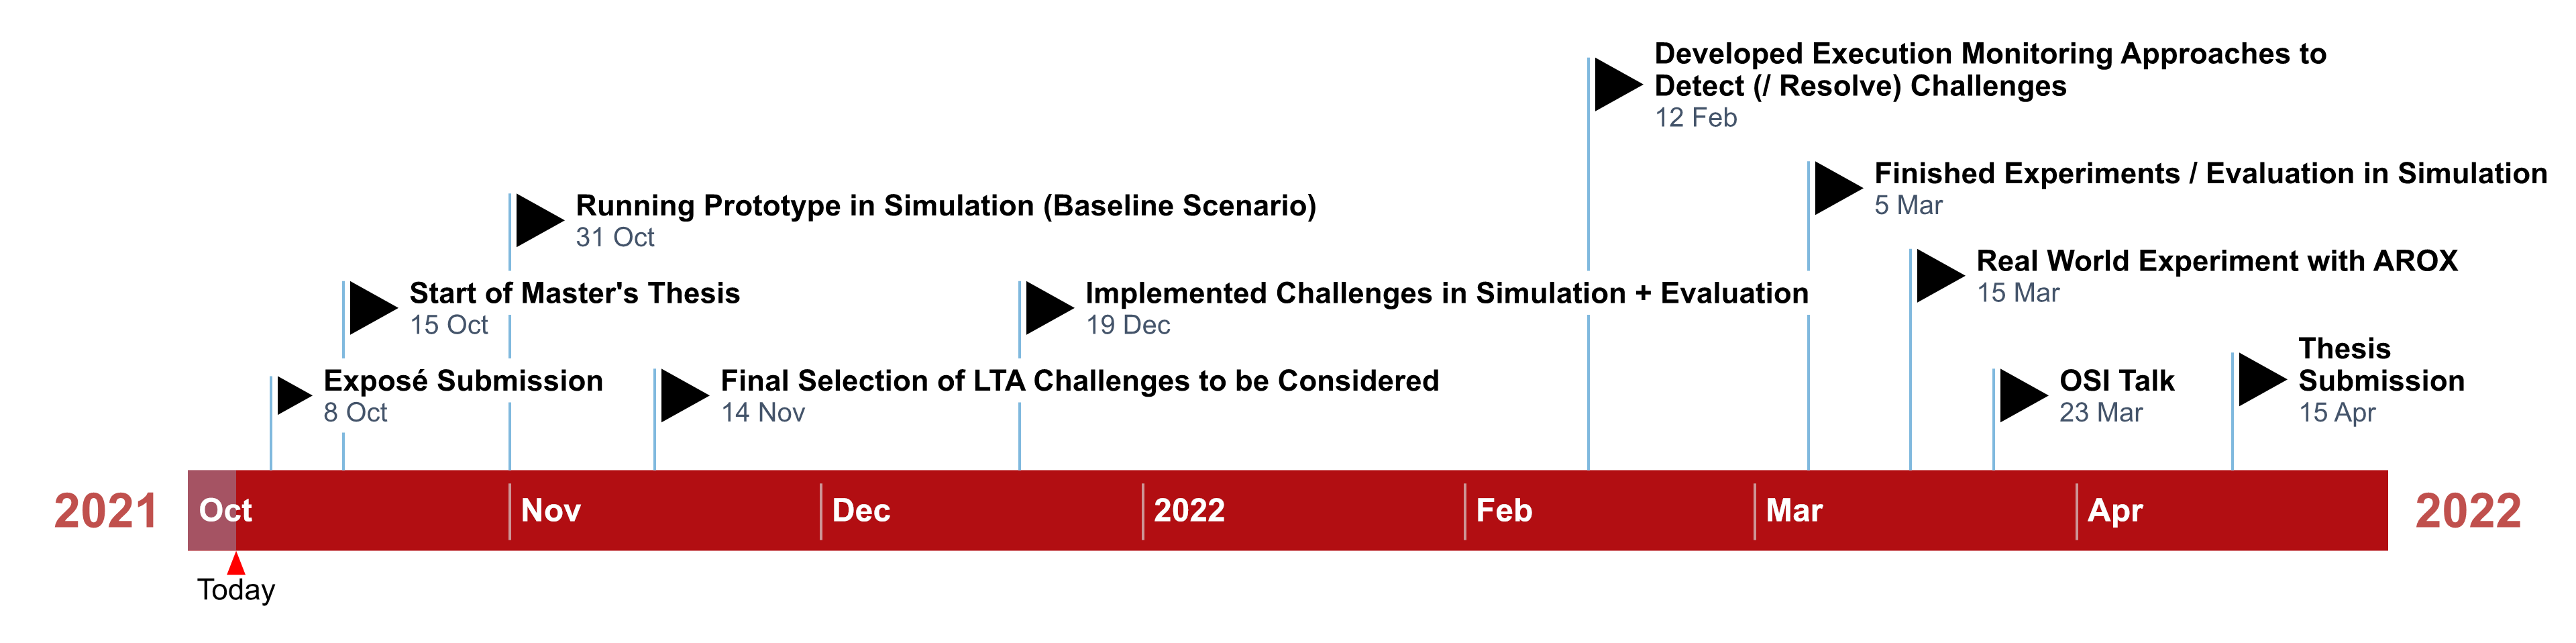
\includegraphics[width=0.95\textwidth]{pics/work_program.png}
    \caption{\textsc{Project Milestones}}
    \label{fig:work_program}
\end{figure}

% DON'T set \bibliographystyle here -- use the documentclass option instead
\bibliography{papers}

\end{document}
